A civil engineer that has recently graduated from the Czech Technical University
encountered an interesting problem and asked us for a help. The problem is more
of economical than engineering nature. The engineer needs to connect several
buildings with an infrastructure. Unfortunately, the investor is not the owner
of all the land between these places. Therefore, some properties have to be
bought first.

The land is divided into a regular ``grid'' of hexagonal parcels, each of them
forms an independent unit and has the same value. Some of the parcels belong to
the investor. These parcels form four connected areas, each containing one
building to be connected with the others. Your task is to find the minimal
number of parcels that must be acquired to connect the four given areas.

\begin{center}
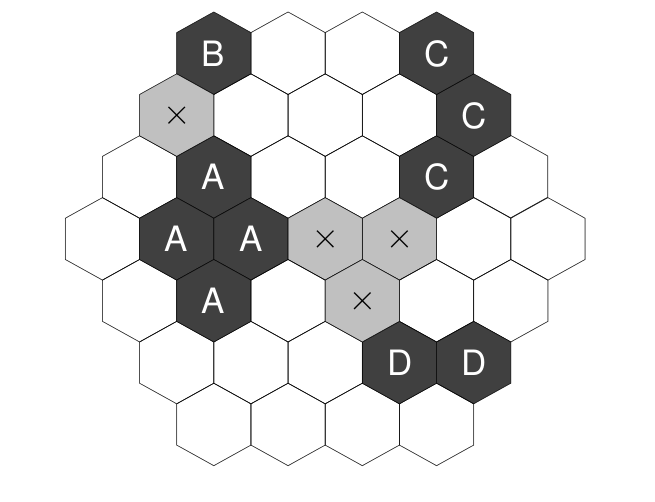
\includegraphics[scale=0.3]{problems/hexagonal/imagens/hex.png}
\end{center}

The whole land also has a hexagonal shape with six sides, each consisting of
exactly $H$ parcels. The above picture shows a land with $H = 4$, parcels with
letters represent the four areas to be connected. In this case, it is necessary
to buy four additional parcels. One of the possible solutions is marked by
crosses.

\subsection*{Input}

The input contains several scenarios. Each scenario begins with an integer
number $H$, which specifies the size of the land, $2 \leq H \leq 20$. Then there
are $2*H - 1$ lines representing individual ``rows'' of the land (always oriented
as in the picture). The lines contain one non-space character for each parcel.
It means the first line will contain $H$ characters, the second line $H + 1$, and
so on. The longest line will be the middle one, with $2*H - 1$ characters. Then
the ``length'' descends and the last line contains $H$ parcels, again.

The character representing a parcel will be either a dot (``.'') for the land
that is not owned by the investor, or one of the uppercase letters ``A'', ``B'',
``C'', or ``D''. The areas of parcels occupied by the same letter will always
be connected. It means that between any two parcels in the same area, there
exists a path leading only through that area.

Beside the characters representing parcels, the lines may contain any
number of spaces at any positions to improve ``human readability'' of the
input. There is always at least one space between two letters (or the
dots). After the land description, there will be one empty line and
then the next scenario begins. The last scenario is followed by a line
containing zero.

\subsection*{Output}

For each scenario, output one line with the sentence ``You have to buy $P$
parcels.'', where $P$ is the minimal number of parcels that must be acquired to
make all four areas connected together.

Areas are considered connected, if it is possible to find a path between them
that leads only through parcels that have been bought.

\begin{table}[!h]
\centering
\begin{tabular}{|l|l|}
\hline
\begin{minipage}[t]{3in}
\textbf{Sample Input}
\begin{verbatim}
4
    B . . C
   . . . . C
  . A . . C .
 . A A . . . .
  . A . . . .
   . . . D D
    . . . .

0
\end{verbatim}
\vspace{1mm}
\end{minipage}
&

\begin{minipage}[t]{3in}
\textbf{Sample Output}
\begin{verbatim}
You have to buy 4 parcels.
\end{verbatim}
\vspace{1mm}
\end{minipage} \\
\hline
\end{tabular}
\end{table}

\newpage
